

\tikzset{every picture/.style={line width=0.75pt}} %set default line width to 0.75pt        

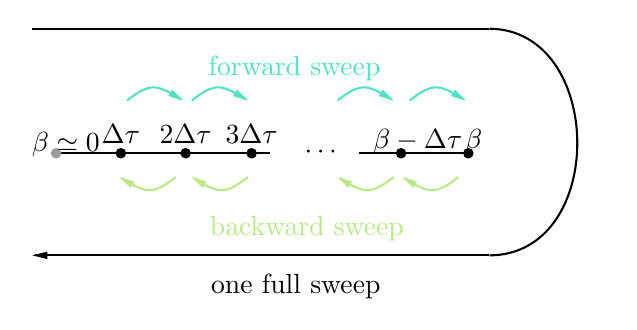
\begin{tikzpicture}[x=0.75pt,y=0.75pt,yscale=-0.6,xscale=0.6]
%uncomment if require: \path (0,300); %set diagram left start at 0, and has height of 300

%Straight Lines [id:da6495692288307713] 
\draw    (90,116) -- (262,116) ;
%Straight Lines [id:da08844155559093347] 
\draw    (142,116) ;
\draw [shift={(142,116)}, rotate = 0] [color={rgb, 255:red, 0; green, 0; blue, 0 }  ][fill={rgb, 255:red, 0; green, 0; blue, 0 }  ][line width=0.75]      (0, 0) circle [x radius= 3.35, y radius= 3.35]   ;
%Straight Lines [id:da767273937626862] 
\draw    (421,116) ;
\draw [shift={(421,116)}, rotate = 0] [color={rgb, 255:red, 0; green, 0; blue, 0 }  ][fill={rgb, 255:red, 0; green, 0; blue, 0 }  ][line width=0.75]      (0, 0) circle [x radius= 3.35, y radius= 3.35]   ;
%Straight Lines [id:da6842453471866836] 
\draw    (333,116) -- (421,116) ;
%Straight Lines [id:da19518547344952264] 
\draw    (194,116) ;
\draw [shift={(194,116)}, rotate = 0] [color={rgb, 255:red, 0; green, 0; blue, 0 }  ][fill={rgb, 255:red, 0; green, 0; blue, 0 }  ][line width=0.75]      (0, 0) circle [x radius= 3.35, y radius= 3.35]   ;
%Straight Lines [id:da270141089403112] 
\draw    (247,116) ;
\draw [shift={(247,116)}, rotate = 0] [color={rgb, 255:red, 0; green, 0; blue, 0 }  ][fill={rgb, 255:red, 0; green, 0; blue, 0 }  ][line width=0.75]      (0, 0) circle [x radius= 3.35, y radius= 3.35]   ;
%Straight Lines [id:da8579502152092178] 
\draw    (367,116) ;
\draw [shift={(367,116)}, rotate = 0] [color={rgb, 255:red, 0; green, 0; blue, 0 }  ][fill={rgb, 255:red, 0; green, 0; blue, 0 }  ][line width=0.75]      (0, 0) circle [x radius= 3.35, y radius= 3.35]   ;
%Straight Lines [id:da9831057926891251] 
\draw [color={rgb, 255:red, 155; green, 155; blue, 155 }  ,draw opacity=1 ]   (90,116) ;
\draw [shift={(90,116)}, rotate = 0] [color={rgb, 255:red, 155; green, 155; blue, 155 }  ,draw opacity=1 ][fill={rgb, 255:red, 155; green, 155; blue, 155 }  ,fill opacity=1 ][line width=0.75]      (0, 0) circle [x radius= 3.35, y radius= 3.35]   ;
%Curve Lines [id:da6761493335679989] 
\draw [color={rgb, 255:red, 80; green, 227; blue, 194 }  ,draw opacity=1 ]   (147,73.67) .. controls (166.5,58.07) and (171.74,61.48) .. (190.53,72.78) ;
\draw [shift={(192,73.67)}, rotate = 210.96] [fill={rgb, 255:red, 80; green, 227; blue, 194 }  ,fill opacity=1 ][line width=0.08]  [draw opacity=0] (12,-3) -- (0,0) -- (12,3) -- cycle    ;
%Curve Lines [id:da7106993363119161] 
\draw [color={rgb, 255:red, 80; green, 227; blue, 194 }  ,draw opacity=1 ]   (199,73.67) .. controls (218.5,58.07) and (223.74,61.48) .. (242.53,72.78) ;
\draw [shift={(244,73.67)}, rotate = 210.96] [fill={rgb, 255:red, 80; green, 227; blue, 194 }  ,fill opacity=1 ][line width=0.08]  [draw opacity=0] (12,-3) -- (0,0) -- (12,3) -- cycle    ;
%Curve Lines [id:da9217626178741651] 
\draw [color={rgb, 255:red, 80; green, 227; blue, 194 }  ,draw opacity=1 ]   (316,73.67) .. controls (335.5,58.07) and (340.74,61.48) .. (359.53,72.78) ;
\draw [shift={(361,73.67)}, rotate = 210.96] [fill={rgb, 255:red, 80; green, 227; blue, 194 }  ,fill opacity=1 ][line width=0.08]  [draw opacity=0] (12,-3) -- (0,0) -- (12,3) -- cycle    ;
%Curve Lines [id:da8930911177321839] 
\draw [color={rgb, 255:red, 80; green, 227; blue, 194 }  ,draw opacity=1 ]   (374,73.67) .. controls (393.5,58.07) and (398.74,61.48) .. (417.53,72.78) ;
\draw [shift={(419,73.67)}, rotate = 210.96] [fill={rgb, 255:red, 80; green, 227; blue, 194 }  ,fill opacity=1 ][line width=0.08]  [draw opacity=0] (12,-3) -- (0,0) -- (12,3) -- cycle    ;
%Curve Lines [id:da8578698860693803] 
\draw [color={rgb, 255:red, 184; green, 233; blue, 134 }  ,draw opacity=1 ]   (413,135.11) .. controls (393.5,150.71) and (388.26,147.3) .. (369.47,136) ;
\draw [shift={(368,135.11)}, rotate = 30.96] [fill={rgb, 255:red, 184; green, 233; blue, 134 }  ,fill opacity=1 ][line width=0.08]  [draw opacity=0] (12,-3) -- (0,0) -- (12,3) -- cycle    ;
%Curve Lines [id:da8070797252206534] 
\draw [color={rgb, 255:red, 184; green, 233; blue, 134 }  ,draw opacity=1 ]   (361,135.11) .. controls (341.5,150.71) and (336.26,147.3) .. (317.47,136) ;
\draw [shift={(316,135.11)}, rotate = 30.96] [fill={rgb, 255:red, 184; green, 233; blue, 134 }  ,fill opacity=1 ][line width=0.08]  [draw opacity=0] (12,-3) -- (0,0) -- (12,3) -- cycle    ;
%Curve Lines [id:da2812724546545875] 
\draw [color={rgb, 255:red, 184; green, 233; blue, 134 }  ,draw opacity=1 ]   (244,135.11) .. controls (224.5,150.71) and (219.26,147.3) .. (200.47,136) ;
\draw [shift={(199,135.11)}, rotate = 30.96] [fill={rgb, 255:red, 184; green, 233; blue, 134 }  ,fill opacity=1 ][line width=0.08]  [draw opacity=0] (12,-3) -- (0,0) -- (12,3) -- cycle    ;
%Curve Lines [id:da6890423553866853] 
\draw [color={rgb, 255:red, 184; green, 233; blue, 134 }  ,draw opacity=1 ]   (186,135.11) .. controls (166.5,150.71) and (161.26,147.3) .. (142.47,136) ;
\draw [shift={(141,135.11)}, rotate = 30.96] [fill={rgb, 255:red, 184; green, 233; blue, 134 }  ,fill opacity=1 ][line width=0.08]  [draw opacity=0] (12,-3) -- (0,0) -- (12,3) -- cycle    ;
%Straight Lines [id:da8340093405550972] 
\draw    (71,16) -- (438,16) ;
%Straight Lines [id:da08632105037669247] 
\draw    (73,198) -- (438,198) ;
\draw [shift={(71,198)}, rotate = 0] [fill={rgb, 255:red, 0; green, 0; blue, 0 }  ][line width=0.08]  [draw opacity=0] (12,-3) -- (0,0) -- (12,3) -- cycle    ;
%Curve Lines [id:da41432957611590804] 
\draw    (438,16) .. controls (531,16.67) and (533,197.67) .. (438,198) ;

% Text Node
\draw (287,115) node [anchor=west] [inner sep=0.75pt]   [align=left] {$\displaystyle \cdots $};
% Text Node
\draw (142,110.6) node [anchor=south] [inner sep=0.75pt]    {$\Delta \tau $};
% Text Node
\draw (194,110.6) node [anchor=south] [inner sep=0.75pt]    {$2\Delta \tau $};
% Text Node
\draw (247,110.6) node [anchor=south] [inner sep=0.75pt]    {$3\Delta \tau $};
% Text Node
\draw (416,94.4) node [anchor=north west][inner sep=0.75pt]    {$\beta $};
% Text Node
\draw (342,94.4) node [anchor=north west][inner sep=0.75pt]    {$\beta -\Delta \tau $};
% Text Node
\draw (68,96.4) node [anchor=north west][inner sep=0.75pt]    {$\beta \simeq 0$};
% Text Node
\draw (210,36) node [anchor=north west][inner sep=0.75pt]  [color={rgb, 255:red, 80; green, 227; blue, 194 }  ,opacity=1 ] [align=left] {forward sweep};
% Text Node
\draw (211,164) node [anchor=north west][inner sep=0.75pt]  [color={rgb, 255:red, 184; green, 233; blue, 134 }  ,opacity=1 ] [align=left] {backward sweep};
% Text Node
\draw (212,211) node [anchor=north west][inner sep=0.75pt]   [align=left] {one full sweep};


\end{tikzpicture}
